\chapter{Systém Apk Analyzer}
\label{chap:apk-analyzer}

Primárnym cieľom tejto diplomovej práce je navrhnúť a implementovať mobilnú aplikáciu pre operačný systém Android, ktorá slúži na analýzu aplikačných balíčkov za účelom získania podrobných informácií o nainštalovaných aplikáciách. Na základe informácií získaných analýzou poskytuje táto mobilná aplikácia možnosť detekcie prebalených a škodlivých aplikácií. 

Za účelom dosiahnutia stanovených cieľov je v rámci práce implementované softvérové riešenie pozostávajúce z mobilnej aplikácie, serverovej časti a centrálnej databázy. Obrázok \ref{fig:systémApkAnalyzer} schematicky znázorňuje koncept vytvoreného systému.

\begin{figure}[htb]
  \begin{center}
    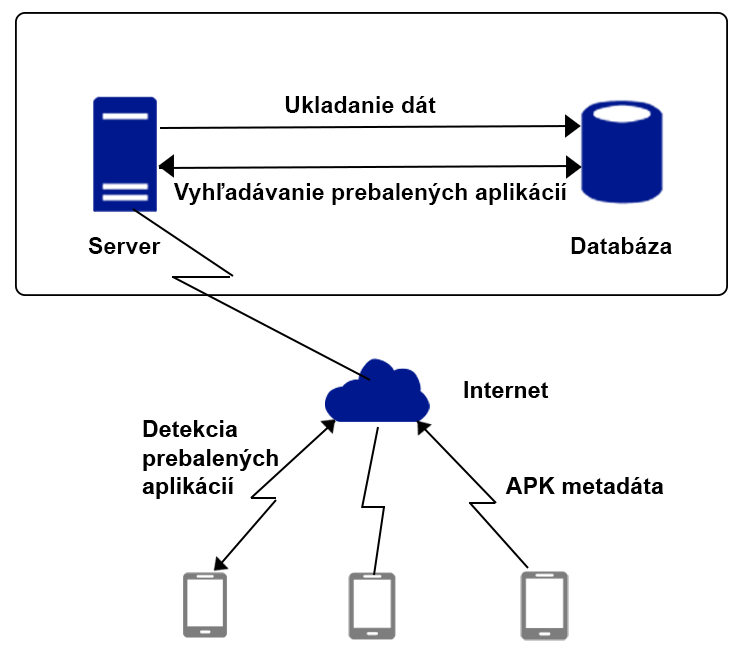
\includegraphics[width=110mm]{images/system-overview.png}
  \end{center}
  \caption{Návrh systému \zv{Apk Analyzer}}
  \label{fig:systémApkAnalyzer}
\end{figure}

\section{Mobilná aplikácia}
Základ systému tvorí mobilná aplikácia \zv{Apk Analyzer}. Aplikácia vykonáva analýzu všetkých nainštalovaných aplikácií v Android zariadení a ponúka možnosť analýzy aplikácií pred ich samotnou inštaláciou. Aplikácia poskytuje užívateľovi detailné informácie o aplikáciách, vrátane možností zobrazenia štatistík o softvérovom obsahu jeho zariadenia a možnosti detekcie prebalených aplikácií. \zv{Apk Analyzer} na pozadí odosiela informácie o aplikáciách na vzdialený server. Tieto informácie sú použité pri tvorbe databázy potrebnej pre detekciu prebalených aplikácií. Detailný popis vytvorenej aplikácie vrátane metód získavania informácií o aplikáciách obsahuje kapitola \label{chap:mobilna-aplikacia}.
.

\section{Server}
Detekcia prebalených aplikácií nie je implementovaná priamo v mobilnej aplikácií, ale na strane zdieľaného servera. Tento dizajn je potrebný z dôvodu implementácie navrhnutej metódy detekcie prebalených aplikácií. Informácie o spôsobe detekcie prebalených aplikácií obsahuje kapitola \ref{chap:metoda-detekcie-apk-analyzer}. Navrhnutá metóda pracuje s rozsiahlou databázou dát o aplikačných balíčkoch. Takáto rozsiahla kolekcia dát nie je zdieľaná medzi mobilnými zariadeniami. Prístup k dátam zabezpečuje centrálny server. 
\newline
\noindent Dôvody komunikácie mobilných zariadení a serveru:
\begin{itemize}
	\item Mobilné zariadenia odosielajú metadáta o ich aplikáciách
	\item Mobilné zariadenia odosielajú požiadavky na analýzu prebalených aplikácií
	\item Mobilné zariadenia dostávajú informácie o výsledkoch analýzy prebalených aplikácií
\end{itemize}
Server poskytuje administrátorom nasledujúce služby:
\begin{itemize}
	\item Rozhranie na správu dát
	\item Vyhľadávanie v databáze aplikácií
	\item Zobrazenie štatistických údajov využitia služby
	\item Zobrayenie výsledkov detekcie prebalených aplikácií spolu s údajmi vysvetlujúcimi rozhodnutie systému
\end{itemize}

\section{Databáza}
Dáta odoslané mobilnými klientami na server sú ukladané v zdieľanom úložisku. Databáza obsahuje metadáta o všetkých aplikáciách odoslaných z mobilných zariadení. Tieto dáta obsahujú všetky kľúčové atribúty potrebné pre detekciu prebalených aplikácií. Spôsob ukladania dát predstavuje dôležitý aspekt pri detekcií prebalených APK balíčkov. Veľká časť operácií potrebných na detekciu prebalených aplikácií je implementovaná pomocou SQL príkazov priamo nad databázou. 
